\chapter{Xây dựng hệ thống} \label{chapter03}

\section{Hệ thống phân loại bệnh trên lá cam}

Hệ thống phân loại bệnh trên lá cam bao gồm 2 mô đun chính: mô đun huấn luyện mô hình và mô đun phân loại bệnh lá cam như hình \ref{fig:system-flowchart}.\par

Mô đun huấn luyện mô hình thực hiện các bước: cơ sở dữ liệu ảnh được trải qua các giải thuật trích đặc trưng (SIFT--BoVW, Color, HOG, GIST, ResNet), tổng hợp véc-tơ đặc trưng (từ các giải thuật trích đặc trưng), huấn luyện mô hình. 

Mô đun phân loại nhận đầu vào là một ảnh được trải qua các giải thuật trích đặc trưng (SIFT--BoVW, Color, HOG, GIST, ResNet), tổng hợp véc-tơ đặc trưng (từ các giải thuật trích đặc trưng), sử dụng mô hình phân loại (được huấn luyện bởi mô đun huấn luyện mô hình) để phân loại. 
 
\begin{figure}[h]
	\centering
	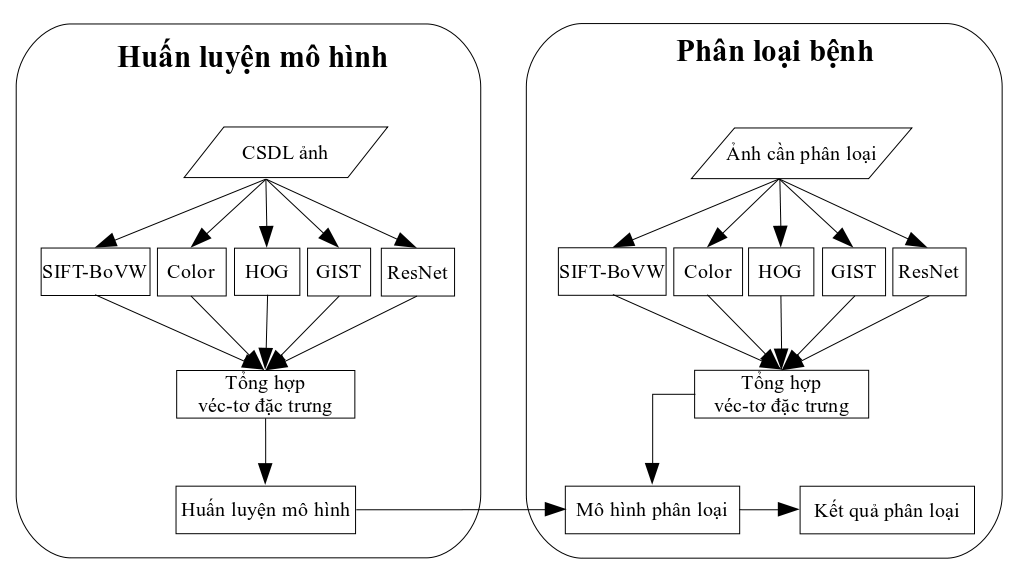
\includegraphics[width=0.9\textwidth]{system-flowchart}
	\caption{Sơ đồ hệ thống phân loại bệnh trên lá cam}
	\label{fig:system-flowchart}
\end{figure}

\section{Thu thập và tổ chức dữ liệu}
\subsection{Thu thập ảnh}
Ảnh lá cam được thu thập từ máy ảnh Panasonic DMC-FH1 độ phân giải 3-Megapixel, độ nhạy sáng (ISO) 400 và tiêu cự 28mm, tại 2 tỉnh Đồng Tháp và Hậu Giang. Một ảnh hợp lệ chỉ chứa một lá cam bệnh, nền không chứa các đối tượng khác, thời gian chụp khi lá cam bắt đầu nhiễm bệnh hoặc đang nhiễm bệnh, chụp trực diện ở phần mặt trên của lá, riêng bệnh rầy phấn trắng do đặc điểm gây bệnh nên sẽ được chụp thêm ở phần mặt dưới của lá.

\subsection{Tổ chức dữ liệu}\label{sub:to-chuc-du-lieu}
Tập các ảnh được tổ chức dưới dạng các thư mục, một thư mục tương ứng là tập hợp các ảnh của một loại bệnh và tên thư mục cũng là tên lớp (hình \ref{fig:dataset}). Mỗi lớp có số lượng ảnh gần ngang bằng nhau, cụ thể, lớp Ghẻ nhám là 142, Là khỏe là 143, Rầy phấn trắng là 141, Vàng lá gân xanh là 142 và Vàng lá thối rễ là 143 ảnh.\par

\begin{figure}[h]
	\centering
	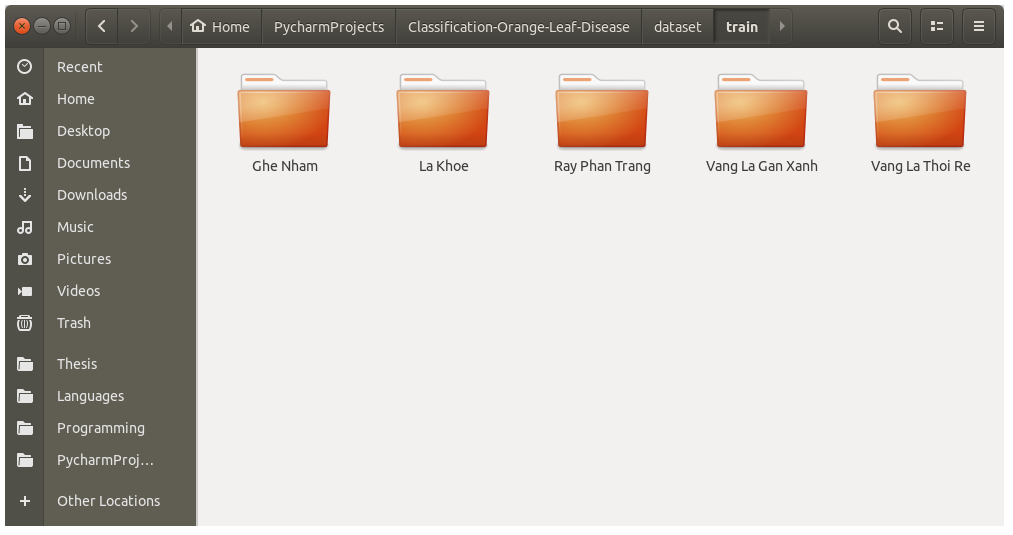
\includegraphics[width=0.8\textwidth]{dataset}
	\caption{Cách tổ chức dữ liệu}
	\label{fig:dataset}
\end{figure}

\section{Trích chọn các đặc trưng}\label{sec:xay-dung-ma-tran}
\subsection{Trích chọn đặc trưng SIFT}
Dựa trên phần cơ sở lý thuyết được giới thiệu ở chương 2, tiến hành xây dựng tập các mô tả của điểm hấp dẫn (keypoint), khởi tạo các tham số mặc định từ giải thuật SIFT, một ảnh đầu vào sau khi qua các bước tính toán sẽ nhận được một véc-tơ 128 thành phần (bins). Bước tiếp theo, chúng tôi áp dụng giải thuật K-Means để gom cụm các mô tả, trong luận văn này chúng tôi tiến hành chọn số lượng cụm là 400 (clusters).  Mô tả trích chọn ở giải thuật SIFT của mỗi ảnh đầu vào sau khi lượng hóa véc-tơ sẽ có 400 thành phần.

\subsection{Trích chọn đặc trưng Color}
Tiếp theo thực hiện trích chọn các đặc trưng Color nhận được một véc-tơ 512 thành phần cho mỗi ảnh, tức là, $8 \times 8 \times 8 = 512$. Tiến hành trích chọn dựa trên ba kênh màu, chia biểu đồ (histogram) có giá trị cường độ trong khoảng 0 đến 255 thành 8 bins cho từng kênh màu (đỏ, xanh lá canh, xanh dương).

\subsection{Trích chọn đặc trưng HOG}
Ảnh đầu vào được đưa về kích thước 80$\times$80 trước khi được tính toán gradient ảnh và biểu đồ gradient, ảnh được chia thành 100 blocks, 8 là kích thước pixel trên mỗi cell (1$\times$1), kích thước bin trên mỗi cell là 9 (bins). Mỗi ảnh đầu vào sẽ nhận được một véc-tơ có 900 thành phần, tức là, $100 \times 9 \times 1 \times 1= 900$.

\subsection{Trích chọn đặc trưng GIST}
Trước tiên ảnh cần được chuẩn hóa về kích thước 128$\times$128, -- Tiền xử lý, tách 3 kênh màu (đỏ, xanh lá cây, xanh dương), biến đổi tỷ lệ lôgarit (giảm độ chênh lệch tỷ lệ các điểm ảnh tối so với các điểm ảnh sáng), thêm các điểm ảnh biên, lọc trắng ảnh (cân bằng năng lượng phổ), lọc chuẩn hóa độ tương phản, xóa các điểm ảnh biên, -- Sinh 20 bộ lọc Gabor để áp dụng lên từng ảnh (đỏ, xanh lá cây, xanh dương, đã được tiền xử lý và chuyển về miền tần số), -- Chia ảnh thành 16 vùng riêng biệt bằng nhau, tính giá trị trên mỗi vùng bằng cách lấy tổng giá trị của các điểm ảnh trên mỗi vùng chia cho số điểm ảnh của vùng, thực hiện lần lược 20 bộ lọc trên 16 vùng của ảnh đỏ, xanh lá cây, xanh dương thu được véc-tơ 960 thành phần, tức là, $16 \times 20 \times 3 = 960$.

\subsection{Trích chọn đặc trưng Residual Networks}
Ảnh đầu vào được chuẩn hóa về kích thước 224$\times$224 trước khi nhận được một véc-tơ đặc trưng có 100352 thành phần tại lớp fully-connected sau khi đã dropout. Bộ tham số của mô hình được huấn luyện sẵn từ tập dữ liệu ImageNet sau đi đã loại bỏ lớp soft-max.

\subsection{Tổng hợp véc-tơ đặc trưng}
Ảnh bệnh sau khi trải qua các bước trích chọn đặc trưng, mỗi giải thuật trích chọn đặc trưng sẽ nhận được một véc-tơ đặc trưng có thành phần (chiều) khác nhau (SIFT--400, Color--512, HOG--900, GIST--960 và Residual Networks--100352), tổng hợp (nối) các véc-tơ tương ứng này ta nhận được một véc-tơ có 103124 thành phần.



\section{Huấn luyện mô hình}
\subsection{Chuẩn bị tập dữ liệu huấn luyện}
Tập dữ liệu gồm 569 ảnh, gồm 5 loại, trong đó 4 loại lá bệnh và 1 loại lá khỏe được tổ chức thành các thư mục (lớp). Sau khi qua bước rút trích các đặc trưng tạo ra dữ liệu dạng bảng mỗi dòng tương ứng là ảnh lá bệnh có 103124 thành phần (chiều) và nhãn là loại bệnh trong hệ thống, dữ liệu đã được xáo trộn ngẫu nhiên trước khi đưa vào huấn luyện. Bảng \ref{tab:train-dataset} thống kê số lượng mẫu trong từng lớp.

\begin{table}[h!]
\caption{Thống kê số lượng mẫu trong tập dữ liệu huấn luyện}
\centering
\begin{tabular}{|c|l|c|c|}
\hline
\textbf{STT} & \textbf{Tên loại bệnh} & \textbf{Nhãn trong hệ thống} & \textbf{Số lượng mẫu} \\ [0.5ex]
\hline \hline
1 & Ghẻ nhám & 0 & 112 \\ 
2 & Lá khỏe & 1 & 115 \\ 
3 & Rầy phấn trắng & 2 & 111 \\ 
4 & Vàng lá gân xanh & 3 & 115 \\ 
5 & Vàng lá thối rễ  & 4 & 116 \\ \hline
\multicolumn{2}{|c|}{ \textbf{Tổng cộng:}} & 5 & 569 \\ \hline
\end{tabular}
\label{tab:train-dataset}
\end{table}

\subsection{Huấn luyện mô hình} \label{sec:training-model}
Trong luận văn này, chúng tôi đề xuất huấn luyện mô hình SVM phân loại bệnh do những ưu điểm vượt trội trong vấn đề phân loại ảnh so với mô hình K láng giềng gần nhất (K-Nearest Neighbour - KNN) \cite{kim12012comparing}. Mô hình SVM được chúng tôi sử dụng hàm nhân Linear vì số chiều của véc-tơ lớn. Chúng tôi cũng điều chỉnh siêu tham số $\gamma$ của hàm nhân Linear và hằng số $C$ (tham số dung hòa lỗi và độ rộng của lề SVM) để có được kết quả cao nhất dựa trên nghi thức kiểm tra chéo từ tập dữ liệu huấn luyện, trong phần tiếp theo chúng tôi cũng sẽ sử dụng nghi thức này để tìm bộ tham số tốt nhất cho mô hình KNN nhằm so sánh hiệu quả so với mô hình SVM. Bộ tham số chúng tôi tìm được là $\gamma = 0.0001$ và $C = 0.01$. 

